\documentclass[main.tex]{subfiles}
\begin{document}

\section{Детерминированные модели в квантовой нотации}\label{ch2}

\subsection{Базовая структура детерминированных моделей}\label{ch2.1}

Для детерминированных моделей мы будем использовать ту же нотацию Дирака. Физическое состояние обозначим $\left|A\right>$, где $A$ может означать некоторый массив не обязательно целых или вещественных чисел, задающих онтологическое состояние. В этом состоянии может находиться наша детерминированная система. Такие состояния сами по себе не образуют гильбертова пространства, поскольку в детерминированной теории у нас нет суперпозиций, но мы можем объявить, что они образуют базис для гильбертова пространства, который мы можем определить [102, 122], решив раз и навсегда, что все онтологические состояния образуют ортонормированное множество: 

\begin{equation}\label{2.1}
	\langle A\mid B\rangle  \equiv \delta_{AB}
\end{equation}

Мы можем позволить этому множеству генерировать гильбертово пространство, если уточним, что имеем в виду, когда говорим о суперпозициях. В гильбертовом пространстве мы теперь вводим квантовые состояния $\left|\psi\right>$ как более общие, чем онтологические состояния:

\begin{equation}\label{2.2}
	 \left|\psi\right> = \sum_A \lambda_A \left|A\right>, \,\,
	 \sum_A |\lambda_A|^2 \equiv 1
\end{equation}

Квантовое состояние может использоваться в качестве шаблонной абстракции для занятий физикой. При этом мы имеем в виду следующее: 

\textit{\textbf{Шаблон} (базовое состояние) - это квантовое состояние вида (\ref{2.2}), описывающее ситуацию, в которой вероятность нахождения нашей системы в онтологическом состоянии $\left|A\right>$ равна $|\lambda_A|^2$. }

Заметим, что $\lambda_A$ может быть комплексным или отрицательным числом, тогда как фаза $\lambda_A$ не играет никакой роли. Несмотря на это, комплексные числа окажутся здесь весьма полезными, как мы увидим позже. Использование квадрата в (\ref{2.2}) и в нашем определении выше, является довольно произвольным выбором; в принципе, мы могли бы использовать другую степень. Здесь мы используем квадраты, потому что это, безусловно, самый полезный выбор; различные степени не повлияли бы на физику, но привели бы к ненужным математическим сложностям. Квадраты гарантируют, что сохранение вероятности равносильно правильной нормализации базового состояния и позволяет использовать унитарные матрицы в наших преобразованиях.  

Иногда мы можем вводить индикаторы $A,B,...$ чтобы представить непрерывные переменные. В этом случае мы имеем непрерывную детерминированную систему; Дельта Кронекера в (\ref{2.1}) заменяется дельтой Дирака и суммы в (\ref{2.2}) будут заменены интегралами. На данный момент мы придерживаемся дискретной нотации. Подчеркнем, что шаблонные состояния не являются онтологическими. Следовательно, у нас пока нет прямой интерпретации для внутренних произведений $\langle\psi_1\mid\psi_2\rangle$, если оба $\left|\psi_1\right>$ и $\left|\psi_2\right>$ являются шаблонными состояниями. Только абсолютные квадраты $\langle A\mid \psi\rangle $ , где $\left<A\right|$ - сопряженное онтологического состояния, обозначают вероятности $|\lambda_A|^2$. Временная эволюция детерминированной модели теперь может быть записана в операторной форме: 

\begin{equation}\label{2.3}
	\left|A(t)\right> = \left|\hat P(t)A(0)\right>
\end{equation}

где $\hat P^{(t)}$ - оператор перестановки. Мы можем записать его как матрицу $P^{(t)}_{AB}$ содержащую только нули и единицы. Тогда(\ref{2.3}) можно записать как матричное уравнение

\begin{align}\label{2.4}
	\left|A(t)\right> = U(t)_{AB}\left|B(0)\right>, &&
	U(t)_{AB} = P^{(t)}_{AB}
\end{align}

По определению элементы матрицы оператора $U(t)$ в этом базисе могут быть только 0 или 1.
На этом этапе очень важно, чтобы мы выбрали $\hat P(t)$ как самый что ни на есть канонический перестановщик, то есть он должен быть обратимым.\footnote{Можно представить детерминированные модели, в которых $\hat P(t)$ необратим, что означает, что два разных онтологических состояния могут развиться в одно и то же состояние. Мы рассмотрим эту возможность позже} Если закон эволюции не зависит от времени, мы имеем

\begin{align}\label{2.5}
	\hat P(t) = (\hat P(\delta t))^{t/\delta t}, && 
	\hat U(t) = (\hat U(\delta t))^{t/\delta t}
\end{align}

где перестановщик $\hat P(\delta t)$ и связаная с ним матрица $\hat U(\delta t)$ описывает эволюцию за кратчайший временной шаг $\delta t$.

Обратите внимание, что никакого вреда не будет, если некоторые элементы в матрице $\hat U(\delta t)_{ab}$ выбраны в качестве унимодулярных комплексных чисел. Однако, обычно это не так важно, так как простое вращение онтологического состояния в комплексной плоскости не имеет физического смысла, но это может быть полезно для математики.
Теперь мы можем сформулировать наше первое важное математическое наблюдение: \textit{квантовые или шаблонные состояния $\left|\psi\right>$ все подчиняются одному и тому же эволюционному уравнению:}

\begin{equation}\label{2.6}
	 \left|\psi(t)\right> = \hat U(t) \left|\psi(0)\right>
\end{equation}

Легко заметить, что вероятности $\left |\lambda\right |^2 $ развиваются, как и ожидалось. Большая часть работы, описанной в этой книге, будет посвящена написанию операторов эволюции $\hat U(t)$ в виде экспонент. То есть нужно найти Эрмитовый оператор $\hat H$ такой, что:

\begin{equation}\label{2.7}
	 \hat U(\delta t) = e^{-i\hat H\delta t},\,so\,that\,\,\,\hat U( t) = e^{-i\hat H t}
\end{equation}


Это делает временную переменную t непрерывной, если первоначально она могла быть только целым числом, кратным $\delta t$ . Найти пример такого оператора на самом деле легко. Если для простоты мы ограничимся шаблонными состояниями $\left|\psi\right>$, ортогональными собственному состоянию $\hat U(t)$ с собственным значением 1, то для (\ref{2.7}) получим решение:  

\begin{equation}\label{2.8}
	\hat H \delta t=\pi-i \sum_{n=1}^{\infty} \frac{1}{n}\left(\hat U(n \delta t)-\hat U(-n \delta t)\right)
\end{equation}

Это уравнение можно проверить с помощью анализа Фурье, см. Часть II. Обратите внимание, что необходимо уточнение: для наименьшего из собственных значений $\left|\O\right>$ (основного состояния) оператора Н справедливо $\hat U\left|\O\right> = \left|\O\right>$ и $\hat H\left|\O\right> = 0$, так что (\ref{2.8}) является недопустимым для такого состояния, но здесь это незначительно (это единственное состояние, для которого (\ref{2.8}) терпит неудачу). Если мы имеем периодический автомат, то уравнение можно заменить конечной суммой, также действительной для состояния с наименьшей энергией. Есть еще одна причина, по которой это не всегда гамильтониан, который мы хотим: его собственные значения всегда будут между 0 и $2\pi/\delta t$, в то время как иногда нам могут пригодиться значения энергии, которые принимают большие значения. Мы делаем вывод, что гамильтониан существует всегда. Повторяем, что онтологические состояния, как и все остальные шаблонные состояния (\ref{2.2}) подчиняются уравнению Шредингера, 

\begin{equation}\label{2.9}
	\frac d {dt} \left|\psi\right> = -i \hat H \left|\psi\right> 
\end{equation}

которое воспроизводит дискретный закон эволюции (\ref{2.7}) во все моменты времени t, которые являются целыми числами, кратными $\delta t$. Поэтому мы всегда воспроизводим \textit{некоторую} "квантовую" теорию!

\subsubsection{Операторы: Бытия, Изменчивости, Сверхневозможности}\label{ch2.1.1}

Мы планируем выделить три типа операторов\footnote{Beables, Changeables and Superimposables}:

\begin{enumerate}
	\item \textit{beables}: они обозначают свойство онтологических состояний, так что beables диагональны в онтологическом базисе $\left\{ \left|A\right>,\,\left|B\right>,\,... \right\}$ гильбертового пространства:

	\begin{equation}\label{2.10}
		\hat{\mathcal{O}} \left|A\right> = \mathcal{O}(A) \left|A\right>
	\end{equation}

	\item \textit{changeables}: операторы, заменяющие онтологическое состояние другим онтологическим состоянием:

	\begin{equation}\label{2.11}
		\hat{\mathcal{O}} \left|A\right> = \left|B\right>
	\end{equation}

	Эти операторы действуют как чистые перестановки.
	\item \textit{superimposables}: они отображают онтологические состояния на суперпозиции онтологических состояний:

	\begin{equation}\label{2.12}
		\hat{\mathcal{O}} \left|A\right> = \lambda_1\left|A\right> + \lambda_2\left|B\right>
	\end{equation}

\end{enumerate}

Теперь мы построим ряд примеров. В Части II мы увидим больше примеров конструкций beables (?бытийных, выполнимых?) операторов.


\subsection{Модель Зубчатого Колеса}\label{ch2.2}

Одной из простейших детерминированных моделей является система, которая может находиться всего в 3 состояниях, называемых (1), (2) и (3). Временной закон эволюции (динамика) состоит в том, что в такт часам (1) эволюционирует в (2), (2) эволюционирует в (3), а состояние (3) эволюционирует в (1). 

\begin{figure}[ht] % вставляем рисунок
\begin{center}
\scalebox{0.4}{
   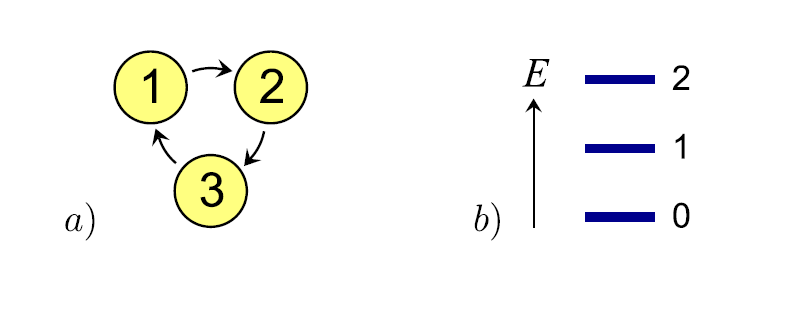
\includegraphics{images/img_2_1.png}
}
\caption{
\label{i2.1}Замкнутая цепочка состояний и ее уровни энергии}
\end {center}
\end {figure}

Пусть часы бьют с временными интервалами $\delta t$. Как было объяснено в предыдущем разделе, мы связываем кеты Дирака с этими состояниями, поэтому у нас есть состояния $\left|1\right>$ , $\left|2\right>$ и $\left|3\right>$. Оператор эволюции $\hat U(\delta t)$ тогда является матрицей:

\begin{equation}\label{2.13}
	\hat U(\delta t)=\left(\begin{array}{lll}{0} & {0} & {1} \\ {1} & {0} & {0} \\ {0} & {1} & {0}\end{array}\right)
\end{equation}

Теперь полезно диагонализировать эту матрицу. Её собственные вектора (состояния) равны $\left|1\right>_H$ , $\left|2\right>_H$ и $\left|3\right>_H$, определяемым как

\begin{equation}\label{2.14}
	\begin{array}{l}{|0\rangle_{H}=\frac{1}{\sqrt{3}}(|1\rangle+|2\rangle+|3\rangle)} \\ {|1\rangle_{H}=\frac{1}{\sqrt{3}}\left(|1\rangle+ e^{2 \pi i / 3}|2\rangle+ e^{-2 \pi i / 3}|3\rangle\right)} \\ {|2\rangle_{H}=\frac{1}{\sqrt{3}}\left(|1\rangle+ e^{-2 \pi i / 3}|2\rangle+ e^{2 \pi i / 3}|3\rangle\right)}\end{array}
\end{equation}

для которых мы имеем

\begin{equation}\label{2.15}
	\hat U(\delta t)\left(\begin{array}{c}{|0\rangle_{H}} \\ {|1\rangle_{H}} \\ {|2\rangle_{H}}\end{array}\right)=\left(\begin{array}{c}{|0\rangle_{H}} \\ {e^{-2 \pi i / 3}|1\rangle_{H}} \\ {e^{-4 \pi i / 3}|2\rangle_{H}}\end{array}\right)
\end{equation}

И запишем в этом базисе:

\begin{align}\label{2.16}
	\hat U = e^{-i\hat H\delta t}, && 
	\hat H =\frac{2\pi}{3\delta t} diag(0,1,2)
\end{align}

В моменты времени t, которые являются целыми кратными $\delta t$, мы имеем в этом базисе,

\begin{equation}\label{2.17}
	\hat U(t) = e^{-i\hat H t}
\end{equation}

но, конечно, это уравнение выполняется в каждом базисе. В терминах онтологического базиса исходных состояний $\left|1\right>$ , $\left|2\right>$ и $\left|3\right>$ гамильтониан (\ref{2.16}) принимает вид:

\begin{equation}\label{2.18}
	\hat H=\frac{2 \pi}{3 \delta t}\left(\begin{array}{ccc}{1} & {\kappa} & {\kappa^{*}} \\ {\kappa^{*}} & {1} & {\kappa} \\ {\kappa} & {\kappa^{*}} & {1}\end{array}\right)
\end{equation}

где $k = -\frac 1 2 + \frac{i\sqrt 3}{6}$, $k^* = -\frac 1 2-\frac{i\sqrt 3}{6}$

Таким образом, мы приходим к выводу, что шаблонное состояние $\left|\psi\right> = \lambda(t)\left|1\right> + \mu(t)\left|2\right> + \nu(t)\left|3\right>$

подчиняется уравнению Шредингера:

\begin{equation}\label{2.19}
	\frac d {dt} \left|\psi\right> = -i \hat H \left|\psi\right> 
\end{equation}

с Гимильтанианом (\ref{2.18}). Таким образом наше уравнение описывает эволюцию модели зубчатого колеса во все моменты времени t, которые являются интегральным кратным $\delta t$. Это является достаточным основанием утверждать, что "квантовая" модель, подчиняющаяся этому уравнению Шредингера, \textit{математически эквивалентна} нашей детерминированной модели зубчатого колеса. Тот факт, что эквивалентность имеет место только при целых кратных $\delta t$, не является ограничением. Представьте себе, что $\delta t$ так же мало, как Планковское время, равное $10^{-43}$ секундам, то, если какие-либо наблюдаемые изменения происходят на гораздо больших временных масштабах, отклонения от онтологической модели будут ненаблюдаемыми. Тот факт, что онтологическая и квантовая модели совпадают при всех целых кратных времени dt, физически важен. Заметим, что исходная онтологическая модель вообще не была определена в нецелочисленное время; мы могли бы просто определить ее, чтобы она была описана квантовой моделью в нецелые времена.   

Собственные значения гамильтониана равны $\frac{2 \pi n}{3 \delta t}$, для n = 0, 1, 2, см. (\ref{i2.1}). Это напоминает атом со спином, который подвергается зеемановскому расщеплению из-за однородного магнитного поля. Можно заключить, что такой атом на самом деле является детерминированной системой с тремя состояниями, или зубчатым колесом, но только в том случае, если был бы идентифицирован "правильный" базис. Читатель может заметить, что это верно только в том случае, если каким-то образом исключаются наблюдения, длящиеся меньше временного шага $\delta t$. Перефразируем. Если быть точным, атом Зеемана - это система, для характеристики которой требуется только 3 (или несколько других целых N) состояний. Это состояния, в которых он находится в три (или N) одинаково разнесенных момента времени. Он возвращается к исходному состоянию после периода $T = N\delta t $.


\subsubsection{Обобщения модели зубчатого колеса: зубчатые колеса с N зубцами}\label{ch2.2.1}

Модель зубчатого колеса можно обобщить как систему, которая переставляет N "онтологических" состояний $\left|n\right>_{ont}$, где $n = 0, ..., N-1$ и N некоторое положительное целое число $> 1$. Предположим, что эволюционный закон заключается в том, что в течиние такта часов происходит переход:

\begin{equation}\label{2.20}
	\left|n\right>_{ont} \rightarrow \left|n + 1 \mod N\right>_{ont}
\end{equation}
             
Эту модель можно рассматривать как универсальное описание любой системы, которая является периодической с периодом N шагов по времени. Состояния в этом эволюционном уравнении рассматриваются как «онтологические» состояния. Модель ничего не говорит об онтологических состояниях между целыми временными шагами. Мы называем это простой периодической моделью зубчатого колеса с периодом N.

Обобщая выкладки из прошлого раздела, выполним дискретное преобразование Фурье для этих состояний:

\begin{equation}\label{2.21}
	|k\rangle_{H} \stackrel{\text { def }}{=} \frac{1}{\sqrt{N}} \sum_{n=0}^{N-1} e^{2 \pi i k n / N}|n\rangle_{\text {ont }}, \quad k=0, \ldots N-1
\end{equation}

\begin{equation}\label{2.22}
	|n\rangle_{\text {ont }}=\frac{1}{\sqrt{N}} \sum_{k=0}^{N-1} e^{-2 \pi i k n / N}|k\rangle_{H}
\end{equation}

Нормируя временной шаг $\delta t$ к единице, имеем


\begin{equation}\label{2.23}
	\hat U(1)|k\rangle_{H}=\frac{1}{\sqrt{N}} \sum_{n=0}^{N-1} e^{2 \pi i k n / N}|n+1 \bmod N\rangle_{\mathrm{ont}}=e^{-2 \pi i k / N}|k\rangle_{H}
\end{equation}

и мы можем сделать вывод

\begin{equation}\label{2.24}
	\hat U(1)=e^{-i \hat H ;} \quad \hat H|k\rangle_{H}=\frac{2 \pi k}{N}|k\rangle_{H}
\end{equation}
                         
Этот Гамильтониан ограничен наличием собственных значений в интервале $[0, 2\pi)$, где нуль входит в интервал, а $2\pi$ - нет. На самом деле, это определение подразумевает, что Гамильтониан является периодическим с периодом $2\pi$, но в большинстве случаев мы будем рассматривать его как ограниченный интервалом. Наиболее интересными физическими случаями будут те, в которых временной интервал очень мал, например, близок к времени Планка, так что высокие значения гамильтониана будут означать, что соответствующие собственные состояния на практике могут считаться несущественными.
В исходном онтологическом базисе матричные элементы гамильтониана имеют вид


\begin{equation}\label{2.25}
	{}_\mathrm{ont}\left\langle m\left|\hat H\right| n\right\rangle_{\mathrm{ont}}=\frac{2 \pi}{N^{2}} \sum_{k=1}^{N-1} k e^{2 \pi i k(m-n) / N}
\end{equation}

Эту сумму мы можем проработать дальше:

\begin{equation}\label{2.26}
	\hat H=\pi\left(1-\frac{1}{N}\right)-\frac{\pi}{N} \sum_{n=1}^{N-1}\left(\frac{i}{\tan (\pi n / N)}+1\right) \hat U(n)
\end{equation}


Обратите внимание, что, в отличие от (\ref{2.8}) это уравнение включает поправки, необходимые для основного состояния. Для других состояний энергии можно проверить, что уравнение (\ref{2.26}) согласуется с уравнением (\ref{2.8}).
Для дальнейшего использования, уравнения (\ref{2.26}) и (\ref{2.8}) без коррекции основного состояния для случая $U(t)\left| \psi\right> = \left| \psi\right> $ можно обобщить до вида, 

\begin{equation}\label{2.27}
	\hat H = C-\frac{\pi i}{T} \sum_{t_{n}>0}^{t_{n}<T} \frac{\hat U\left(t_{n}\right)}{\tan \left(\pi t_{n} / T\right)} \stackrel{T \rightarrow \infty}{\longrightarrow} C-i \sum_{t_{n} \neq 0} \frac{\hat U\left(t_{n}\right)}{t_{n}}
\end{equation}


где C - (большое) константа, T - период, а $t_n = n\delta t$ - это множество моментов времени, в которые оператор $U(t_n)$ имеет определенное значение. Отметим, что это сумма, а не интеграл, поэтому, когда значения времени очень плотны, гамильтониан имеет тенденцию становиться очень большим. Кажется, не существует простого предельного континуума. Тем не менее, во второй части мы попытаемся его построить.
 
Опять же, если мы введем уравнение Шредингера $\frac d {dt} \left|\psi\right>_t = -i \hat H \left|\psi\right>_t  $ и граничное условие $\left|\psi\right>_{t=0} = \left|n_0\right>_{ont}$, то это состояние подчиняется детерминированному закону эволюции (\ref{2.20}) в целочисленные моменты времени t. Если мы возьмем суперпозиции состояний $\left|n_0\right>_{ont}$ и интерпретацию комплексных коэффициентов по правилу Борна, то уравнение Шредингера по-прежнему правильно описывает эволюцию вероятностей Борна.

Интересно отметить, что энергетический спектр (\ref{2.24}) часто встречается в физике: это спектр атома с полным угловым моментом $J = \frac 1 2 (N-1)$ и магнитным моментом $\mu$ в слабом магнитном поле: Зеемановский атом. Мы видим, что после дискретного преобразования Фурье (\ref{2.21}) атом Зеемана можно рассматривать как простейшую детерминированную систему, которая переходит от одного состояния в другое в дискретных временных интервалах, посещая в общей сложности N состояний.

Как и в атоме Зеемана, мы можем рассмотреть вариант добавления конечной универсальной величины $\delta E$ к Гамильтониану. Здесь имеет место эффект вращения всех состояний с комплексной амплитудой $e^{-i \delta E}$ после каждого временного шага. Для простого зубчатого колеса это может показаться безобидной модификацией, не влияющей на физику, но ниже мы увидим, что эффект добавления такой константы может стать весьма значительным позже.
Обратите внимание, что если мы введем какое-либо возмущение для атома Зеемана, в результате которого энергетические уровни будут разделены на интервалы, которые больше не равны. Тогда наша модель больше не будет вести себя как зубчатое колесо. Такие системы будет намного сложнее описать в детерминированной теории; они должны рассматриваться как части гораздо более сложного мира.

\subsubsection{Наиболее общие детерминированные, обратимые во времени, конечные модели}\label{ch2.2.2}

Обобщая конечные модели, обсуждавшиеся ранее в этой главе, рассмотрим теперь модель с конечным числом состояний и произвольным законом эволюции времени. Начнем с некоторого состояния $\left|n_0\right>_{ont}$ и проследим за его развитием. После некоторого конечного числа, скажем, $N_0$, временных шагов, система вернется к $\left|n_0\right>_{ont}$. Однако не все состояния $\left|n_0\right>_{ont}$ могут быть достигнуты. Итак, если мы начнем с любого из оставшихся состояний, скажем, $\left|n_1\right>_{ont}$, то будет достигнут новый ряд состояний, и периодичность может быть другим числом, $N_1$. Продолжим, пока все существующие состояния модели не будут достигнуты. Таким образом, наиболее общая модель будет описана как набор простых периодических моделей зубчатого колеса с изменяющимися периодичностями, но все они работают с одним и тем же универсальным временным шагом $\delta t$, который мы могли бы нормализовать на единицу; см. рис.\ref{i2.2}.




\begin{figure}[ht] % вставляем рисунок
	\begin{center}
		\scalebox{0.4}{
		   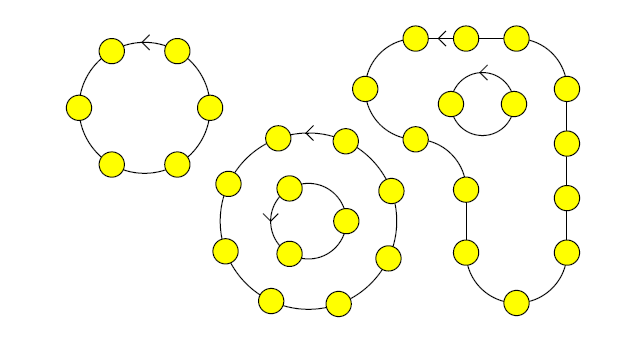
\includegraphics{images/img_2_2.png}
		}
		\caption{
		\label{i2.2} Пример более общей конечной, детерминированной, обратимой во времени модели}
	\end {center}
\end {figure}

\begin{figure}[ht] % вставляем рисунок
	\begin{center}
		\scalebox{0.4}{
		   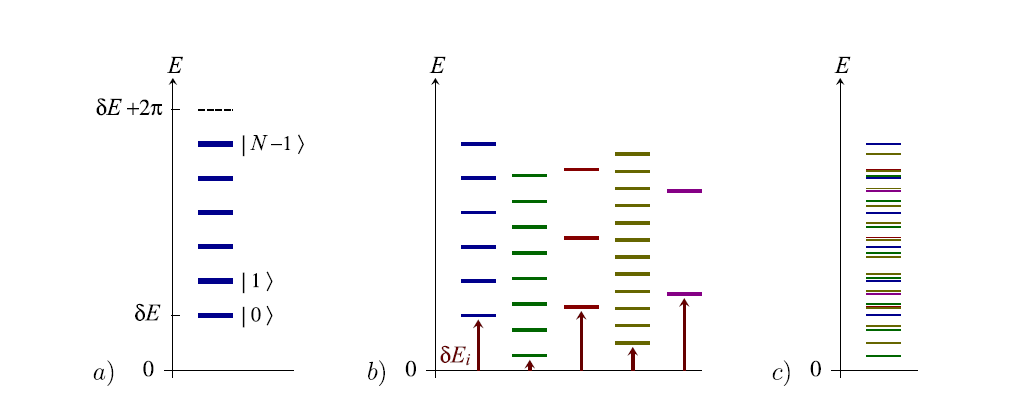
\includegraphics{images/img_2_3.png}
		}
		\caption{
		\label{i2.3} \textbf{a} Энергетический спектр простой периодической модели зубчатого колеса. $\delta E$-произвольный сдвиг энергии. \textbf{b} Энергетический спектр модели, изображенной на рис. \ref{i2.2}, где объединены несколько простых моделей зубчатых колес. Каждое отдельное зубчатое колесо $i$ может быть сдвинуто на произвольную величину $\delta E_i$. \textbf{c} Собирая эти энергетические уровни вместе, мы получим спектр универсальной конечно-элементной модели}
	\end {center}
\end {figure}

Рис. \ref{i2.2} пример более общей конечной детерминированной обратимой модели.

На рисунке \ref{i2.3} показаны уровни энергии простой периодической модели зубчатого колеса (слева), комбинации простых периодических моделей зубчатого колеса (в центре) и наиболее общей детерминированной, обратимой во времени, конечной модели (справа). Обратите внимание, что теперь мы сместили уровни энергии всех зубчатых колес на $\delta E_i$. Это разрешено, потому что индекс $i$, указывающий нам, в каком зубчатом колесе мы находимся, является консервативной величиной, поэтому эти сдвиги не имеют физического эффекта. Однако мы наблюдаем радикальные последствия, когда объединяем спектры в один, см. \ref{i2.3}c.

Рисунок \ref{i2.3} ясно показывает, что энергетический спектр конечной дискретной детерминированной модели может быстро стать довольно сложным.\footnote{Должно быть самоочевидно, что обсуждаемые модели, представленные на рисунках, являются всего лишь простыми примерами; реальная Вселенная будет бесконечно сложнее, чем они. Один критик нашей работы недоумевал: "почему эта модель с 31 состоянием? Что такого особенного в числе 31?" Ничего, конечно, это просто пример, чтобы проиллюстрировать, как работает математика} Возникает следующий вопрос: дан любой тип квантовой системы, энергетический спектр которой можно вычислить. Можно ли определить детерминированную модель, которая имитирует квантовую модель? В какой степени при этом нужно жертвовать локальностью? Существуют ли классы детерминированных теорий, которые можно сопоставить с классами квантовых моделей? Что из этого было бы потенциально интересно?



\end{document}
